\documentclass[12pt,draftcls,onecolumn]{IEEEtran}
%\documentclass[onecolumn]{IEEEtran}

\usepackage{amsmath}
\usepackage{amsthm}
\usepackage{amssymb}  % assumes amsmath package installed
\usepackage{algorithmic}
\usepackage{algorithm}
\usepackage{cite}
\usepackage{color}
\usepackage{comment}
\usepackage{epsfig}
\usepackage{float}
\usepackage{graphicx}
\usepackage{multicol}
\usepackage{subfigure}
\usepackage{setspace}
\usepackage{comment}
\usepackage{subfig} % for subfigures
\usepackage{caption}



\newtheorem{theorem}{Theorem}[section]
\newtheorem{lemma}[theorem]{Lemma}
\newtheorem{proposition}[theorem]{Proposition}
\newtheorem{corollary}[theorem]{Corollary}
\newtheorem{remark}[theorem]{remark}

\begin{document}

\title{Path Planning of Webot Satisficing Experiment ---- Workspace and C-Target Construction  }


\author{  Min Zheng \\  \today}

\date{\today}

% make the title area
\maketitle



%\IEEEpeerreviewmaketitle

%%%%%%%%%%%%%%%%%%%%%%%%%%%%%%%%%%%%%%%%%%%%%%%%%%%%%%%%%%%%%%%%%%%%%%%%%%%%%%
This project considers the integrated navigation and control of an unmanned ground vehicle(UGV) deployed to visually classify multiple targets in an obstacle-populated environment. 
This report describes the problem setup and the contruction of the $\mathcal{C}_{Target}$ . 

\section{Workspace construction} 

The workspace is the same as the one used for active satisficing human studies. 
The UGV and 30 target objects are in the same environment that consists of four rooms, denoted as the region-of-interest (ROI).
Similar to the human studies, there are 30 targets, denoted as $\mathcal{T} = \{\mathcal{T}_i; i = 1,2,...30; \mathcal{T} \subset W \}$.
The targets are considered as points.
A two-dimensional representation from the webot environment was extracted, and the workspace is constructed in MatLab, as shown in the figure below  (Figure \ref{fig:2}). 


The construction of workspace is built in an object oriented manner with classes of obstacles, targets and robot, each has properties and functionalities.  
Note that the table and the chairs are treated differently from other obstacles.
Since their top surfaces are higher than the robot, only their legs will be considered as obstacles. 


\begin{figure}[p]
\centering
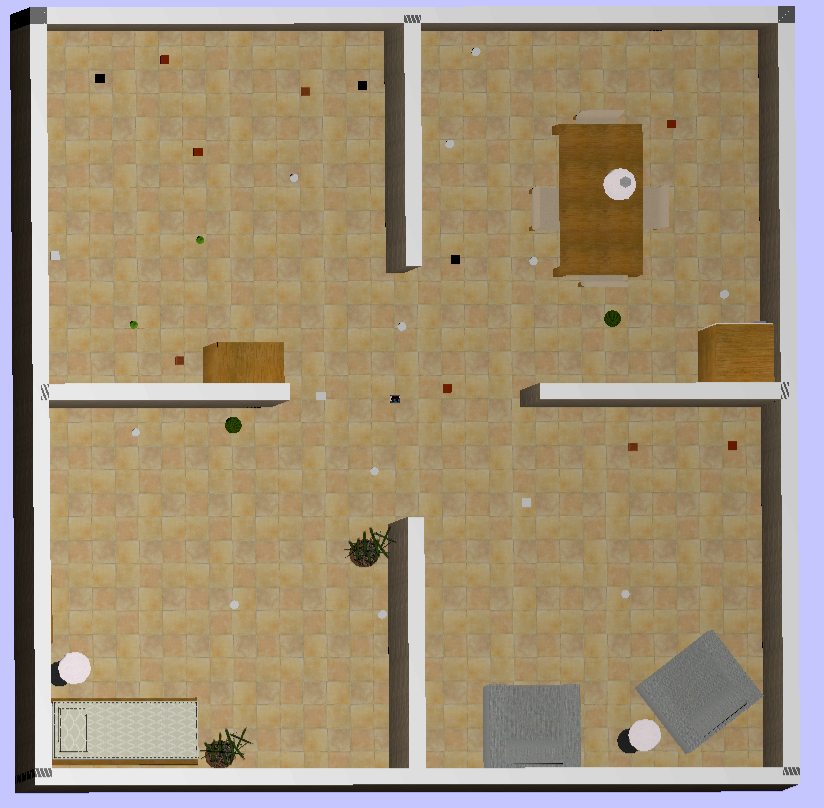
\includegraphics[width=10cm]{figures/webotTop}
  \caption{Top view of the webot environment}
  \label{fig:1}
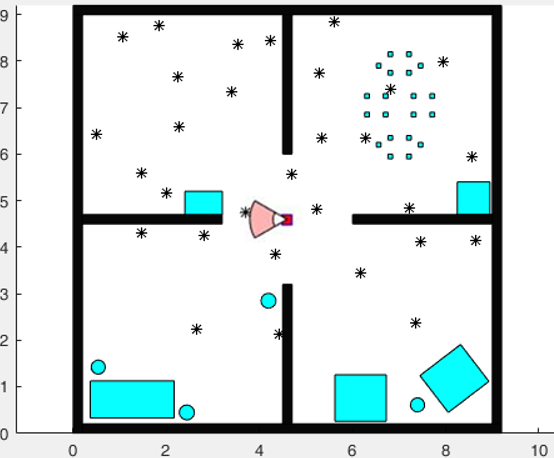
\includegraphics[width=13cm]{figures/newWorld}
  \caption{2D representation built in MatLab. Obstacles are represented by colored regions, and targets represented by the stars. The UGV is  the red square, while its FOV is the red area within the fan shape.}
  \label{fig:2}
\end{figure}



\clearpage


%%%%%%%%%%%%%%%%%%%%%%%%%%%%%%%%%%%%%%%%%%%%%%%%%%%%%%%%%%%%%%%%%%%%%%%%%%%%%%
\section{UGV's specs and FOV} 


The UGV sensor in the webot environment has platform geometry $\mathcal{A}$, and FOV geometry $S \subset \mathbb{R}^2 $. 
The dimension of UGV is 0.12m x 0.10m in 2D.
Its translation step is 0.01m, and rotation step is $\pi/12$ .
The UGV configuration is described in  (Figure \ref{fig:1}).
The configuration vector is defined as $q \equiv [x  \quad  y  \quad  \theta]^T$.



In order to combine with Zeyu's visual classification project, the FOV was determined based on requirement of  images taken. 
A successful classification requires the image to be taken within a minimum and a maximum distance, denoted by $d_{min}$ and  $d_{max}$. 
In human tests, the open angle of FOV for the on board camera is $\alpha =\pi/4 $. 
Therefore the same  $\alpha$ is used here.
Also, in the visual classification problem, Ryan took all the pictures from 0.3m.
If the picture is taken less than that distance, the target object is not guaranteed to be completely within the camera view.
Meanwhile, in the human tests software setup, the robot must be within 1m from the target to  measure or classify.
In such manner, the range of distance from target is conservatively set within $d_{min} = 0.3m$ and  $d_{max}=0.8 m$.
In order to better work with the visual classification, these parameters, especially $d_{max}$ may be subject to changes due to the highly sensitive manner of visual classifier. 
For example, it may be affected by whether the visual classifier allows multiple objects to appear in the view. 

\begin{figure}
 \centering
  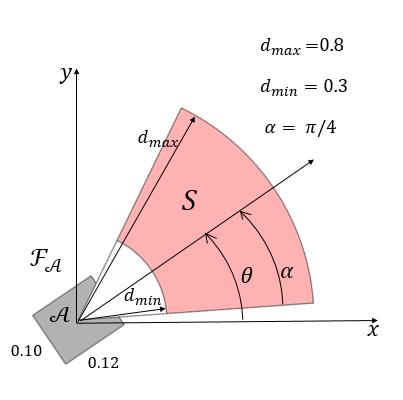
\includegraphics[width=8cm]{figures/FOV}
  \caption{Configuration and FOV of the UGV.}
  \label{fig:3}
\end{figure}


\clearpage






%%%%%%%%%%%%%%%%%%%%%%%%%%%%%%%%%%%%%%%%%%%%%%%%%%%%%%%%%%%%%%%%%%%%%%%%%%%%%%
\section{$\mathcal{C}_{free}$} 


Assume that the UGV can freely rotate. Thus  $ \alpha  \in (-\pi $ , $\pi) $.
In x-y plane, a location is defined to be in $\mathcal{C}_{free}$ if the UGV can freely rotate around its center, which is at the given location.
The locations where some subsets of all possible $ \alpha$ are be allowed is discarded from $\mathcal{C}_{free}$, considering the problem of getting stuck. 
Given the geometry of the UGV, it requires that the bounding circle of the UGV (Figure \ref{fig:3}) does not intersect with any obstacles.
The result $\mathcal{C}_{free}$ is shown in Figure \ref{fig:6}.

\begin{figure}
 \centering
  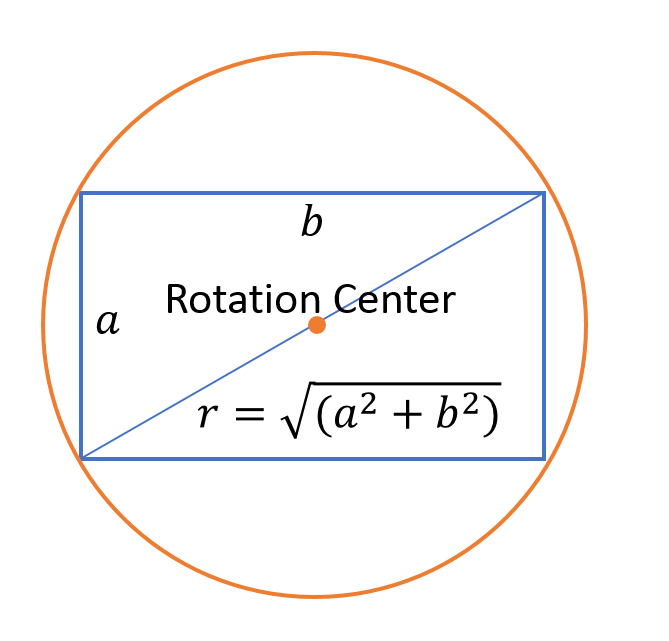
\includegraphics[width=8cm]{figures/rot_demo}
  \caption{The area(orange circle) swept by rotating the UGV(blue rectangle) around  its center. }
  \label{fig:3}
\end{figure}

\begin{figure*}[htp]
  \centering
  \subfigure[ $\mathcal{C}_{free}$ for the whole world map]{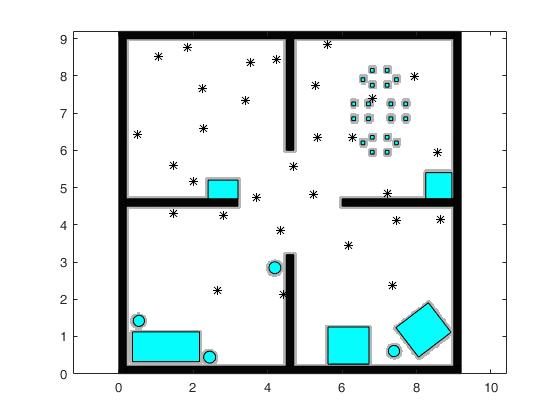
\includegraphics[width=12cm]{figures/Cfree}}\quad
  \subfigure[zoomed-in demonstration of $\mathcal{C}_{free}$, where the center of the circle represents the UGV center location, so that the ]{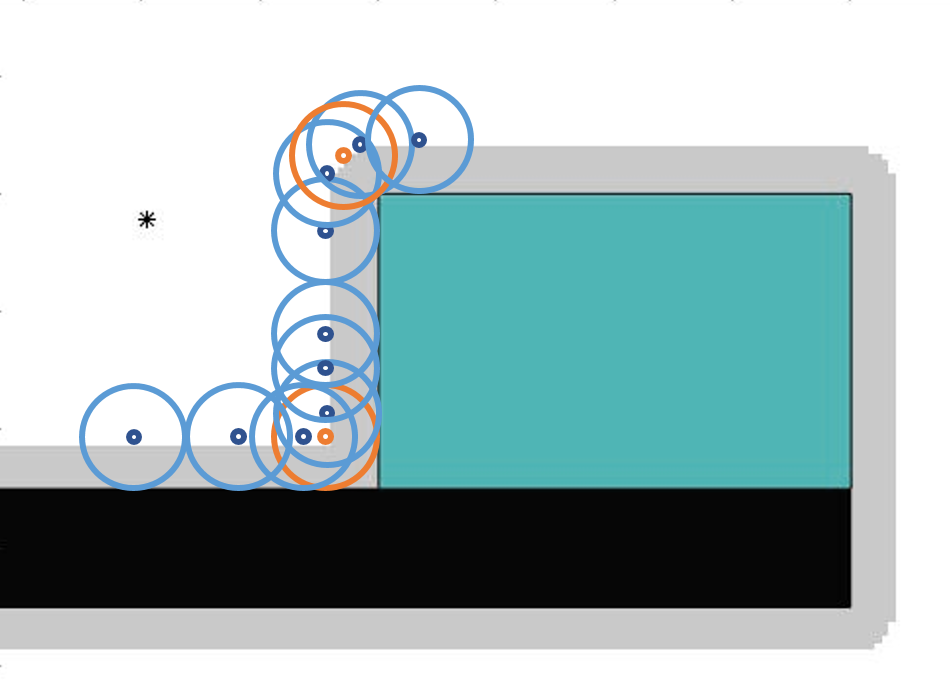
\includegraphics[width=8cm]{figures/Cfree_demo1}}
  \caption{ $\mathcal{C}_{free}$  of the given world map denoted by white region. Grey area is not in  $\mathcal{C}_{free}$ }
  \label{fig:6}
\end{figure*}


\clearpage


%%%%%%%%%%%%%%%%%%%%%%%%%%%%%%%%%%%%%%%%%%%%%%%%%%%%%%%%%%%%%%%%%%%%%%%%%%%%%%
\section{$\mathcal{C}_{Target}$} 


Assume that the UGV camera is mounted at the center the UGV and always face the same direction as the UGV.
$\mathcal{C}_{Target}$  is defined so that the target $\mathcal{T}_i$ in $\mathcal{W}$ maps  in the robot's configuration space  $\mathcal{C}_{free}$ to the C-target region  $\mathcal{CT}_i = \{q \in \mathcal{C}_{free}    |    \mathcal{S}(q) \cap \mathcal{T}_i  \neq  \emptyset \}$.
A simple $x-y$ plane demonstration (Figure \ref{fig:4}) shows the effect of the distance to the target.
In (a), the robot is within $\mathcal{C}_{Target}$, since the target is in the robot's FOV when it faces $-\pi/2$.
In (b), the robot is not in $\mathcal{C}_{Target}$, and it can not detect the target no matter how it rotates at its current position. 

Also, the visibility problem is introduced to deal with the case that the camera view is blocked by obstacles.
That is, a target must be in the FOV of the given UGV configuration, and at the same time, if a line is drawn between the robot and the target, such a line must not cross any obstacle, demonstrated in  (Figure \ref{fig:7}).
If this criteria is met, such a UGV configuration is defined as in the  $\mathcal{C}_{target}$.

The C-Target is plotted for the workspace (Figure \ref{fig:12}).
A zoom-in example is shown in (Figure \ref{fig:8}.





\begin{figure}
 \centering
  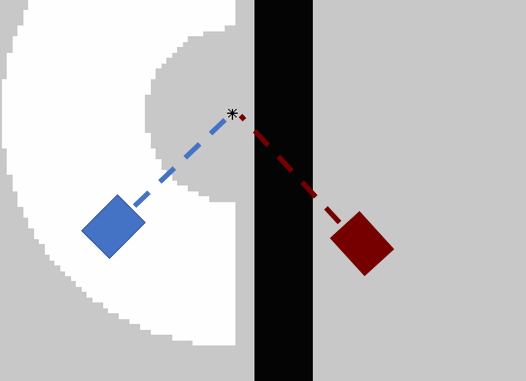
\includegraphics[width=5cm]{figures/visibility_eg}
  \caption{Example of visibility problem handling for a target near the wall. The blue and red rectangles denote the UGV configuration. The dash line denotes the direction the robot is facing. It is also used in the visibility handling. The blue configuration is in C-Target, but the red is not since its view is blocked by the obstacle.}
  \label{fig:7}
\end{figure}



\begin{figure*}[htp]
  \centering
  \subfigure[robot is in C-target]{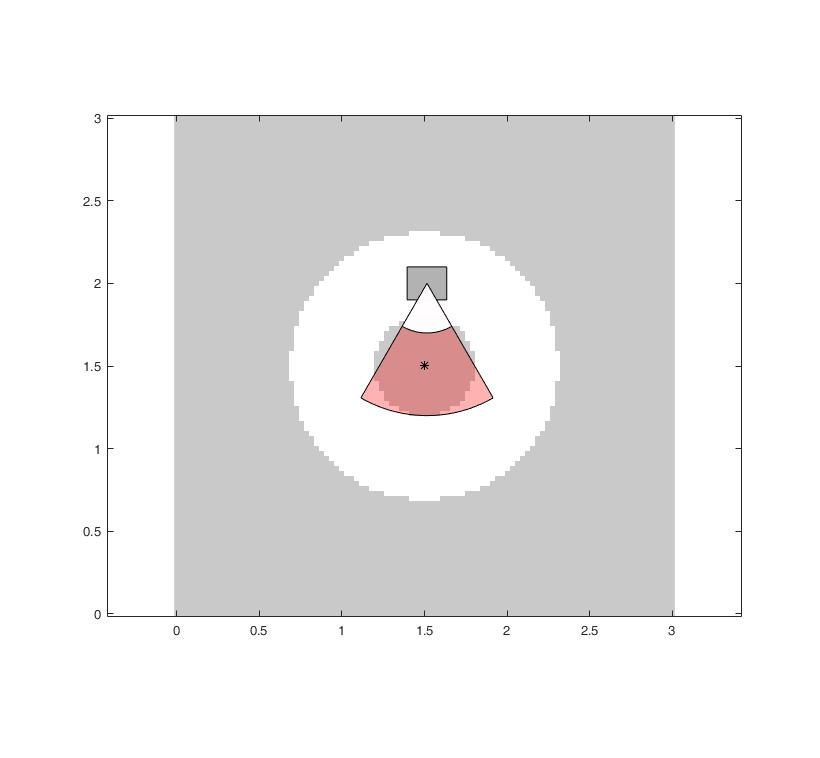
\includegraphics[width=9cm]{figures/oneTargetTrue}}\quad
  \subfigure[robot is not in C-target]{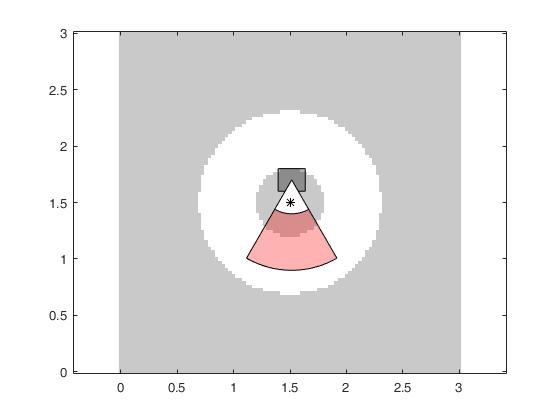
\includegraphics[width=9cm]{figures/oneTargetFalse}}
  \caption{Example of C-target with one target. C-target denoted by white area, and the star denotes the target. The target must fall in the red region(robot FOV) to be classified or measured. In both examples, the UGV is facing $\theta = -\pi/2$}
  \label{fig:4}
\end{figure*}


%\begin{figure}
% \centering
%  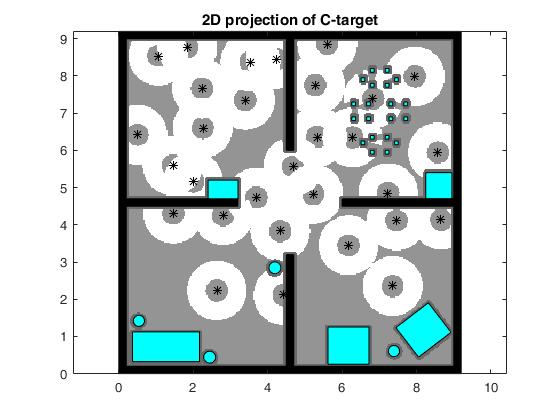
\includegraphics[width=15cm]{figures/CTarget_v2}
%  \caption{x-y projection of C-Target, which is denoted by white.}
%  \label{fig:6}
%\end{figure}





\begin{figure*}[htp]
  \centering
  \subfigure[ ]{\includegraphics[width=13cm]{figures/ctarget_p2}}\quad
  \subfigure[ ]{\includegraphics[width=13cm]{figures/ctarget_p}}\quad
  \caption{ Perspective view of $\mathcal{C}_{target}$}
  \label{fig:9}
\end{figure*}

\begin{figure*}[htp]
  \centering
  \subfigure[$x-y$  view]{\includegraphics[width=14cm]{figures/ctarget_xy}}
 \subfigure[$x-\theta$  view]{\includegraphics[width=10cm]{figures/ctarget_xtheta}}
  \caption{ $\mathcal{C}_{target}$}
  \label{fig:12}
\end{figure*}



\begin{figure*}[htp]
  \centering
  \subfigure[ perspective view]{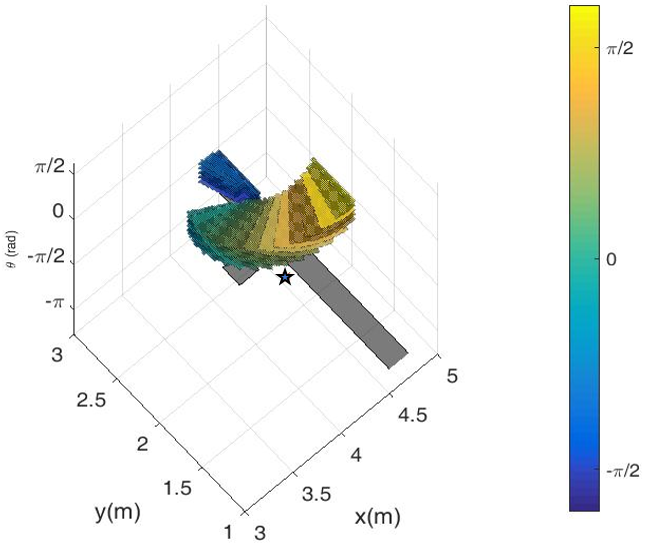
\includegraphics[width=10cm]{figures/ctarget_demo_p}}\quad
  \subfigure[$x-y$  view ]{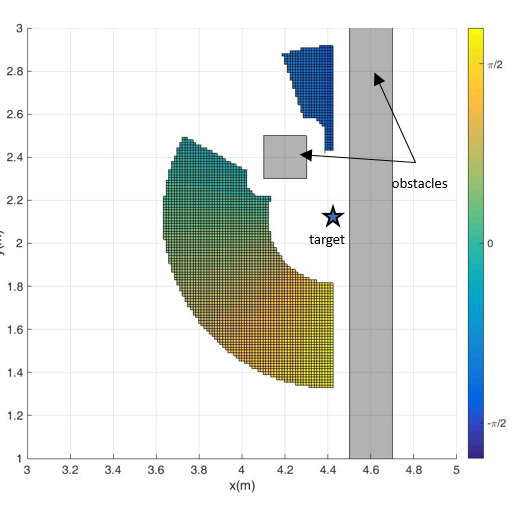
\includegraphics[width=8cm]{figures/ctarget_demo_xy}}\quad
  \subfigure[$x-\theta$  view  and $y-\theta$  view]{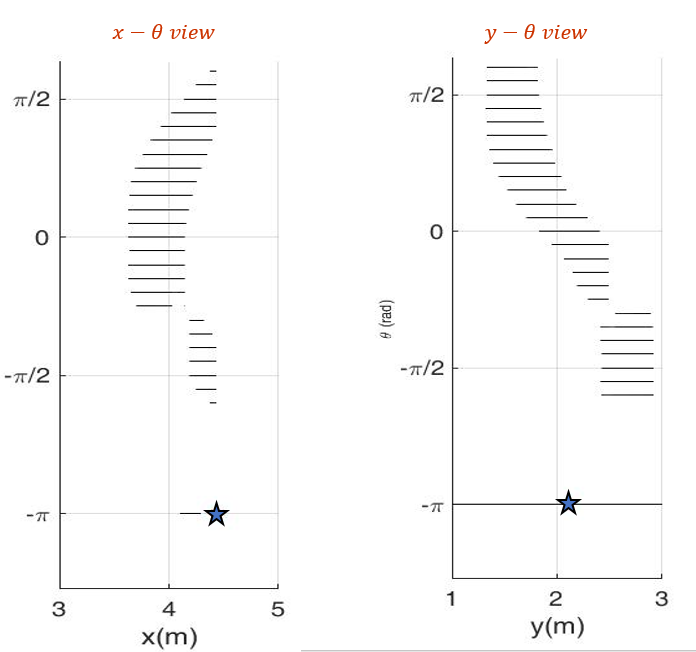
\includegraphics[width=8cm]{figures/ctarget_demo_xytheta}}
  \caption{ An example zoom-in of $\mathcal{C}_{target}$}
  \label{fig:8}
\end{figure*}


\end{document}
